\documentclass[12pt]{article}
\usepackage{graphicx}
\usepackage{amsmath}
\usepackage{float}
\usepackage{booktabs}
\usepackage{hyperref}
\usepackage{verbatim}

\title{\textbf{Experiment 2: Email Classification using Naïve Bayes and K-Nearest Neighbors}}
\author{Pradeep Kumar R}
\date{}

\begin{document}

\maketitle

\section*{Goal and Purpose}
\begin{itemize}
  \item \textbf{Goal:} To categorize emails as either Spam or Ham using machine learning algorithms.
  \item \textbf{Purpose:} Develop and assess Naïve Bayes and KNN models using metrics such as accuracy, precision, recall, F1-score, and ROC analysis. Apply 5-Fold Cross-Validation to measure model robustness.
\end{itemize}

\section*{Key Libraries Utilized}
\begin{itemize}
  \item \texttt{pandas, numpy, matplotlib, seaborn}
  \item \texttt{sklearn.model\_selection} – train\_test\_split, cross\_val\_score, KFold
  \item \texttt{sklearn.naive\_bayes} – GaussianNB, MultinomialNB, BernoulliNB
  \item \texttt{sklearn.neighbors} – KNeighborsClassifier
  \item \texttt{sklearn.metrics} – classification\_report, confusion\_matrix, roc\_curve, auc
  \item \texttt{sklearn.preprocessing} – StandardScaler, MinMaxScaler
\end{itemize}

\section*{Python Implementation}
\begin{verbatim}
import pandas as pd
import numpy as np
import matplotlib.pyplot as plt
import seaborn as sns

from sklearn.model_selection import train_test_split, cross_val_score, KFold
from sklearn.preprocessing import MinMaxScaler, StandardScaler
from sklearn.metrics import accuracy_score, precision_score, recall_score, f1_score, confusion_matrix, roc_curve, auc, classification_report

from sklearn.naive_bayes import GaussianNB, MultinomialNB, BernoulliNB
from sklearn.neighbors import KNeighborsClassifier

# Dataset Loading
df = pd.read_csv("/content/spambase_csv.csv")
print(df.isnull().sum().sum())

# Feature and Label Separation
X = df.iloc[:, :-1]
y = df.iloc[:, -1]

# Feature Scaling
scaler = StandardScaler()
X_scaled = scaler.fit_transform(X)

# Data Visualization
sns.countplot(x=y)
plt.title("Email Label Distribution")
plt.xticks([0, 1], ['Ham', 'Spam'])
plt.show()

df.iloc[:, :5].hist(figsize=(10, 6))
plt.suptitle("Feature Distribution Overview")
plt.show()

# Train-Test Splitting
X_train, X_test, y_train, y_test = train_test_split(X_scaled, y, test_size=0.2, random_state=42, stratify=y)

# Preprocessing for Naïve Bayes
X_train_std = StandardScaler().fit_transform(X_train)
X_test_std = StandardScaler().fit_transform(X_test)
X_train_mnb = MinMaxScaler().fit_transform(X_train)
X_test_mnb = MinMaxScaler().fit_transform(X_test)

# Gaussian Naïve Bayes
gnb = GaussianNB()
gnb.fit(X_train_std, y_train)
y_pred = gnb.predict(X_test_std)
print("\nGaussianNB Results:")
print(classification_report(y_test, y_pred))

# Bernoulli Naïve Bayes
bnb = BernoulliNB()
bnb.fit(X_train_std, y_train)
y_pred = bnb.predict(X_test_std)
print("\nBernoulliNB Results:")
print(classification_report(y_test, y_pred))

# Multinomial Naïve Bayes
mnb = MultinomialNB()
mnb.fit(X_train_mnb, y_train)
y_pred = mnb.predict(X_test_mnb)
print("\nMultinomialNB Results:")
print(classification_report(y_test, y_pred))

# KNN for different k values
for k in [3, 5, 7]:
    knn = KNeighborsClassifier(n_neighbors=k)
    knn.fit(X_train, y_train)
    y_pred = knn.predict(X_test)
    print(f"\nKNN (k={k}) Results:")
    print(classification_report(y_test, y_pred))

# Model Evaluation Function
def evaluate_model(model, name):
    y_pred = model.predict(X_test)
    y_prob = model.predict_proba(X_test)[:, 1] if hasattr(model, 'predict_proba') else None
    acc = accuracy_score(y_test, y_pred)
    prec = precision_score(y_test, y_pred)
    rec = recall_score(y_test, y_pred)
    f1 = f1_score(y_test, y_pred)
    print(f"\n{name} Metrics:\nAccuracy: {acc:.2f}, Precision: {prec:.2f}, Recall: {rec:.2f}, F1-score: {f1:.2f}")

    cm = confusion_matrix(y_test, y_pred)
    sns.heatmap(cm, annot=True, fmt='d', cmap='Blues')
    plt.title(f"{name} Confusion Matrix")
    plt.xlabel("Predicted")
    plt.ylabel("Actual")
    plt.show()

    if y_prob is not None:
        fpr, tpr, _ = roc_curve(y_test, y_prob)
        plt.plot(fpr, tpr, label=f"{name} (AUC = {auc(fpr, tpr):.2f})")
        plt.xlabel('False Positive Rate')
        plt.ylabel('True Positive Rate')
        plt.title(f"{name} ROC Curve")
        plt.legend()
        plt.grid()
        plt.show()

evaluate_model(GaussianNB().fit(X_train, y_train), "GaussianNB")
evaluate_model(KNeighborsClassifier(n_neighbors=5).fit(X_train, y_train), "KNN (k=5)")

# Cross-Validation using K-Folds
kfold = KFold(n_splits=5, shuffle=True, random_state=42)
models = {
    'GaussianNB': GaussianNB(),
    'KNN (k=5)': KNeighborsClassifier(n_neighbors=5),
}

for name, model in models.items():
    scores = cross_val_score(model, X_scaled, y, cv=kfold)
    print(f"{name} Cross-Validation Accuracy: {np.mean(scores):.4f} ± {np.std(scores):.4f}")
\end{verbatim}

\section*{Results and Observations}

\subsection*{Data Exploration}
\begin{figure}[H]
    \centering
    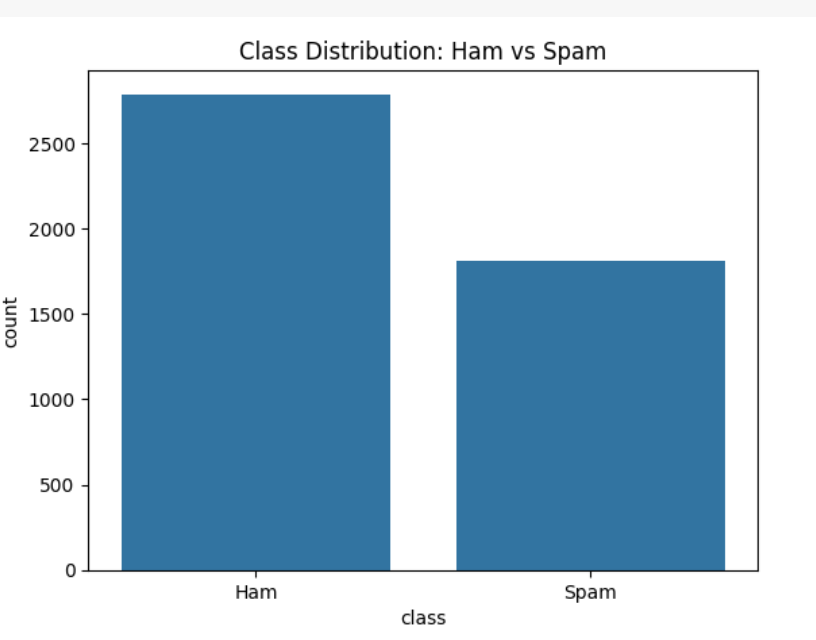
\includegraphics[width=0.6\linewidth]{image1.png}
    \caption{Email Classes: Spam vs Ham}
\end{figure}

\begin{figure}[H]
    \centering
    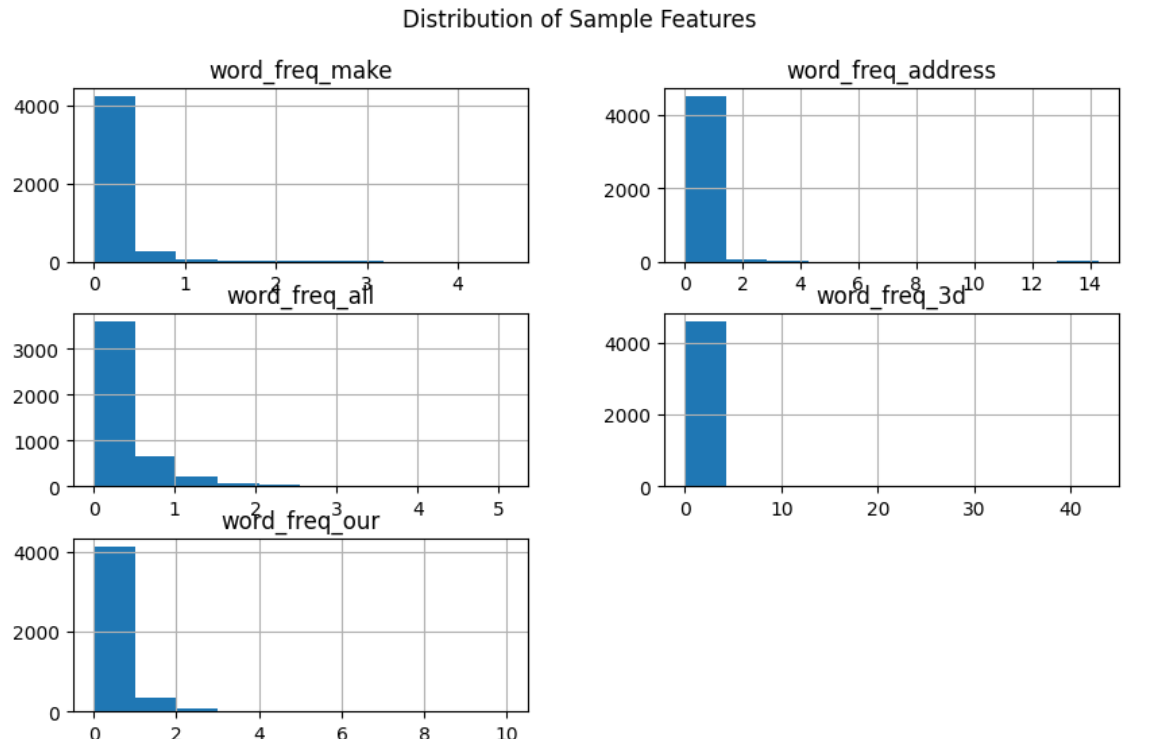
\includegraphics[width=0.8\linewidth]{image2.png}
    \caption{Histogram of Selected Features}
\end{figure}

\subsection*{Naïve Bayes Classifier Metrics}
\textbf{GaussianNB:}\\
Accuracy: 0.83, Precision: 0.71, Recall: 0.96, F1-Score: 0.82

\begin{figure}[H]
    \centering
    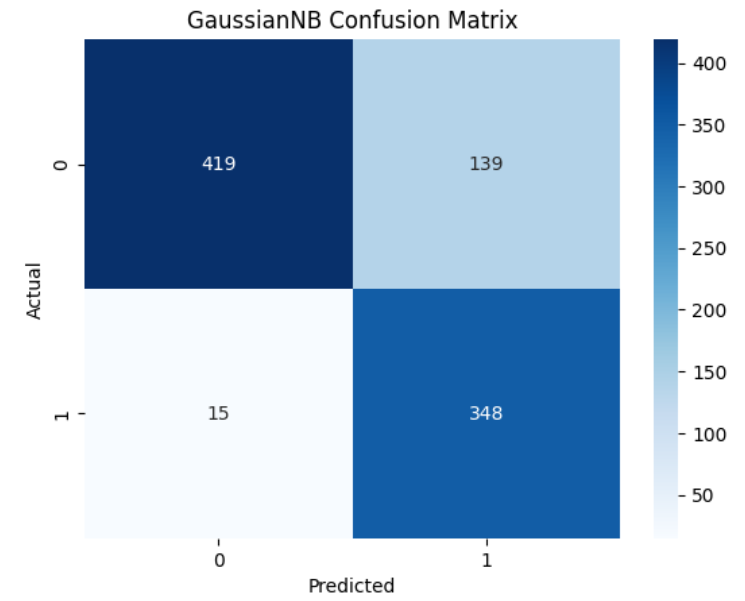
\includegraphics[width=0.5\linewidth]{image3.png}
    \caption{Confusion Matrix - GaussianNB}
\end{figure}

\begin{figure}[H]
    \centering
    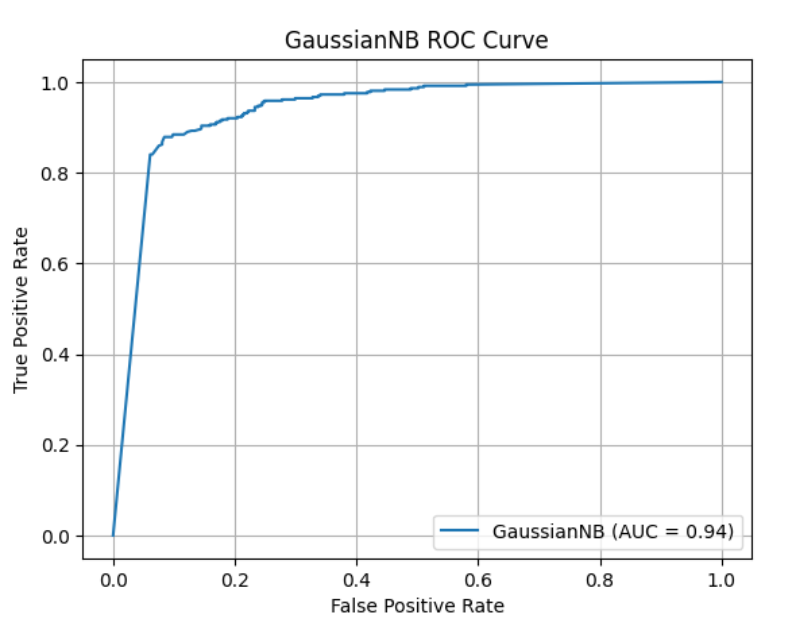
\includegraphics[width=0.6\linewidth]{image4.png}
    \caption{ROC Curve - GaussianNB}
\end{figure}

\subsection*{K-Nearest Neighbors (k=5)}
Accuracy: 0.91, Precision: 0.89, Recall: 0.87, F1-Score: 0.88

\begin{figure}[H]
    \centering
    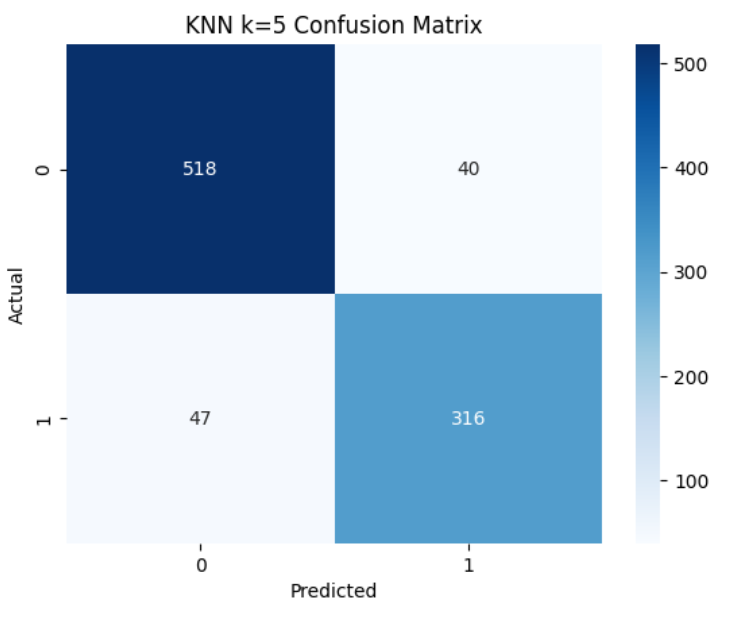
\includegraphics[width=0.5\linewidth]{image5.png}
    \caption{Confusion Matrix - KNN (k=5)}
\end{figure}

\begin{figure}[H]
    \centering
    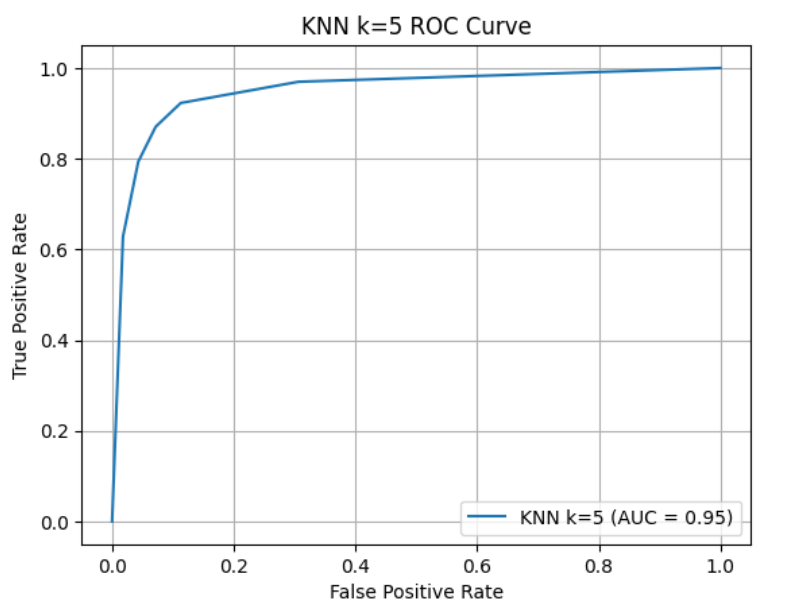
\includegraphics[width=0.6\linewidth]{image6.png}
    \caption{ROC Curve - KNN (k=5)}
\end{figure}

\subsection*{Cross Validation Summary}
\begin{itemize}
  \item GaussianNB Mean Accuracy: 0.8153 ± 0.0142
  \item KNN (k=5) Mean Accuracy: 0.9085 ± 0.0113
\end{itemize}

\section*{Comparison Tables}

\subsection*{Naïve Bayes Variants}
\begin{table}[H]
\centering
\begin{tabular}{lcccc}
\toprule
Model & Accuracy & Precision & Recall & F1 Score \\
\midrule
Gaussian NB & 0.83 & 0.71 & 0.96 & 0.82 \\
Multinomial NB & 0.91 & 0.88 & 0.88 & 0.88 \\
Bernoulli NB & 0.90 & 0.90 & 0.83 & 0.87 \\
\bottomrule
\end{tabular}
\end{table}

\subsection*{KNN with Various k}
\begin{table}[H]
\centering
\begin{tabular}{ccccc}
\toprule
k & Accuracy & Precision & Recall & F1 Score \\
\midrule
3 & 0.90 & 0.88 & 0.87 & 0.87 \\
5 & 0.91 & 0.89 & 0.87 & 0.88 \\
7 & 0.91 & 0.89 & 0.87 & 0.88 \\
\bottomrule
\end{tabular}
\end{table}

\subsection*{K-Fold Cross Validation (k=5)}
\begin{table}[H]
\centering
\begin{tabular}{lcc}
\toprule
Model & Mean Accuracy & Standard Deviation \\
\midrule
GaussianNB & 0.8153 & 0.0142 \\
KNN (k=5)  & 0.9085 & 0.0113 \\
\bottomrule
\end{tabular}
\end{table}

\section*{Insights Gained}
\begin{itemize}
  \item Applied supervised learning techniques to differentiate between spam and non-spam emails.
  \item Evaluated models using key metrics and plotted ROC curves for probabilistic models.
  \item Understood the impact of preprocessing and hyperparameter tuning (e.g., value of k in KNN).
  \item Utilized k-fold cross-validation to validate the generalization performance of classifiers.
\end{itemize}

\end{document}
